Comparing the given equation with the form:
\begin{align}
\label{eq:solutions/3/4/1/eq:conic_quad_form}
\vec{x}^T\vec{V}\vec{x}+2\vec{u}^T\vec{x}+f=0
\end{align}
We get:
\begin{align}
\vec{x}^T\myvec{1 & 0\\0 & -1}\vec{x}+2\myvec{-2 & -3}\vec{x}-6=0 \label{eq:solutions/3/4/1/2.0.2}
\intertext{where,}
\vec{V}=\myvec{1 & 0 \\0 & -1}\label{eq:solutions/3/4/1/eq:2.0.3}\\
\vec{u}=\myvec{-2 \\ -3}\label{eq:solutions/3/4/1/eq:2.0.4}\\
f=-6\label{eq:solutions/3/4/1/eq:2.0.5}
\end{align}
Here, $ \mydet{\vec{V}}=-1$. Since $ \mydet{\vec{V}}<0$ the given equation represents a hyperbola with center:
\begin{align}
\vec{c}&=-\vec{V}^{-1}\vec{u}=\myvec{2\\-3}
\end{align}

The characteristic equation of $\vec{V}$ is:
\begin{align}
\mydet{V-\lambda\vec{I}} = 0\\
\mydet{1-\lambda & 0 \\ 0 & -1-\lambda} = 0\\
\implies \lambda^2 -1 = 0
\label{eq:solutions/3/4/1/eq:asymptotes_char}\\
\lambda_{1}= 1,
\lambda_{2}= -1
\end{align}
Finding the eigen vector matrix $\vec{P}$ such that $\vec{P}^T=\vec{P}^{-1}$.      For $\lambda_1=1$

\begin{align}
    (\vec{V}-\lambda_1 \vec{I})\vec{p}
    _1=0\\
    \myvec{0 & 0 \\0 &-2 }\vec{p}_1=0 \\
    \implies \vec{p}_1=\myvec{1 \\ 0} \\
%    \text{[Choosing Orthonormal eigen vectors]} \nonumber
\end{align}
For $\lambda_2=-1$
\begin{align}
    (\vec{V}-\lambda_2 \vec{I})\vec{p}_2=0\\
    \myvec{2 & 0 \\0 &0 }\vec{p}_2=0 \\
    \implies \vec{p}_2=\myvec{0 \\ 1} \\
    \text{[Choosing Orthonormal eigen vectors]} \nonumber\\
    \vec{P}=\myvec{ \vec{p}_1& \vec{p}_2}=\myvec{1&0 \\0& 1}
\end{align}

By affine transformation $\vec{x} = \vec{P}\vec{y}+\vec{c} $,  Equation \eqref{eq:solutions/3/4/1/eq:conic_quad_form} can be written in the form:
\begin{align} 
\vec{y}^T\vec{D}\vec{y} =  \vec{u}^T\vec{V}^{-1}\vec{u} -f \\
\intertext{where,}
\vec{D} = \myvec{\lambda_1 & 0\\ 0 & \lambda_2},
\label{eq:solutions/3/4/1/eq:quad_form_hyper}
\end{align}
Thus, we can write:
\begin{align}
    \lambda_1y_1^2 -\brak{-\lambda_2}y_1^2 = \vec{u}^T\vec{V}^{-1}\vec{u} -f \label{eq:solutions/3/4/1/eq:2.0.17}
\end{align}
The equation \eqref{eq:solutions/3/4/1/eq:2.0.17} represents a modified hyperbola, The equation of the asymptotes for \eqref{eq:solutions/3/4/1/eq:2.0.17} is:
\begin{align} 
\myvec{\sqrt{\abs{\lambda_1}} & \pm \sqrt{\abs{\lambda_2}}}\vec{y} = 0 \label{eq:solutions/3/4/1/eq2.0.21}
\end{align} 
Putting the values of $\lambda_1$ and $\lambda_2$ in equation \eqref{eq:solutions/3/4/1/eq2.0.21}, we get the two asymptotes for \eqref{eq:solutions/3/4/1/eq:2.0.17}:
\begin{align} 
\myvec{1 & 1}\vec{y} = 0 \\
\myvec{1 & -1}\vec{y} = 0
\end{align} 
These are the asymptotes of our modified hyperbola. The asymptotes of our original hyberbola in equation \eqref{eq:solutions/3/4/1/2.0.2} can be obtained using:
\begin{align} 
%\label{eq:solutions/3/4/1/eq:quad_form_pair}
\myvec{\sqrt{\abs{\lambda_1}} & \pm \sqrt{\abs{\lambda_2}}}\vec{P}^T\brak{\vec{x}-\vec{c}} = 0
\label{eq:solutions/3/4/1/eq:2.0.20}
\end{align} 
Putting the values of $\lambda_1$, $\lambda_2$ and $\vec{P}$  in equation \eqref{eq:solutions/3/4/1/eq:2.0.20}, we get the equations of the asymptotes of the original hyperbola with center at $\Vec{c}$:
\begin{align} 
    \myvec{1 &-1}\myvec{1&0 \\0& 1}\brak{\vec{x}+\myvec{2 \\-3}}=0\\
    \implies \boxed{\myvec{1 &-1}\Vec{x}=5} \label{eq:solutions/3/4/1/2.0.26}\\
    \myvec{1 & 1}\myvec{1&0 \\0& 1}\brak{\vec{x}+\myvec{2 \\-3}}=0\\
     \implies \boxed{\myvec{1 &1}\Vec{x}=-1} \label{eq:solutions/3/4/1/2.0.28}
\end{align}

\begin{figure}[ht!]
    \centering
    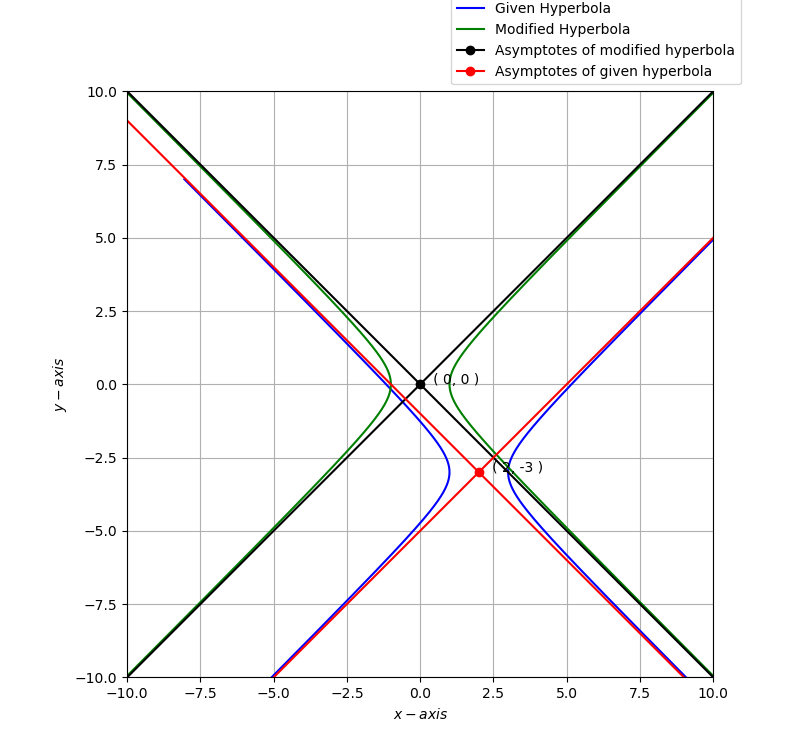
\includegraphics[width=11cm]{./solutions/3/4/1/Figure_1.png}
    \caption{Plot of the Asymtotes.}
    \label{eq:solutions/3/4/1/Plot of the Asymtotes}
\end{figure}
